\section{Formater les partitions existantes et les utiliser pour l'installation}
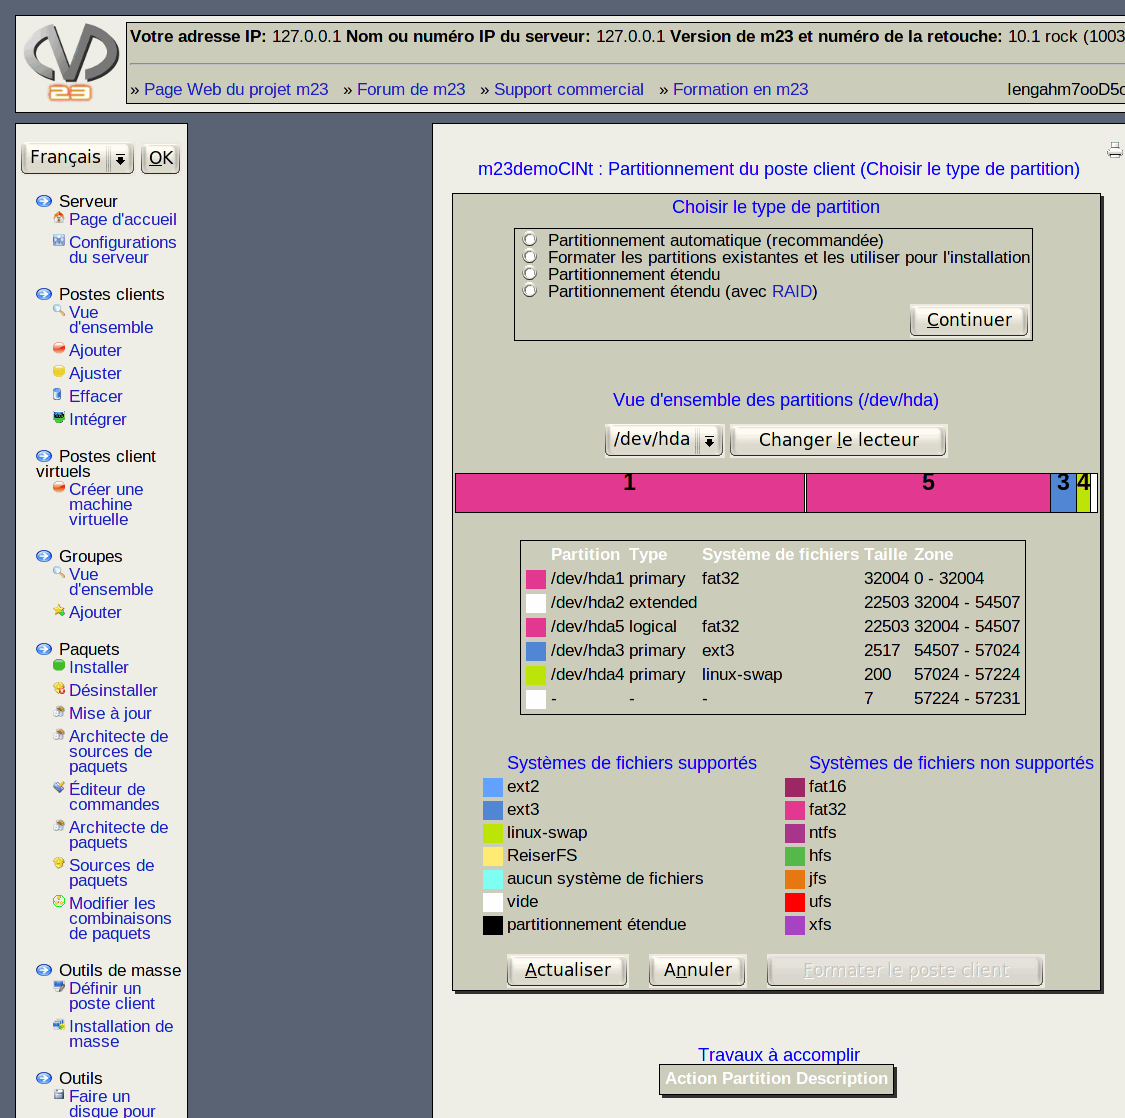
\includegraphics[scale=0.4]{/mdk/doc/manual/screenshots/fr/fdisk-existing.png} \\
Cette option vous offre la possibilit\'e de formater \`a nouveau des partitions existantes et de les employer pour l'installation. Vous devez s\'electionner deux partitions - la premi\`ere pour l'installation du syst\`eme d'exploitation et la deuxi\`eme pour l'espace pour les fichiers d'\'echange (swap).\\
\subsection{Proc\'ed\'e \'etape par \'etape:}
\begin{enumerate}
\item Choisissez \textit{$\ll$Formater les partitions existantes et les utiliser pour l'installation$\gg$}
\item S\'electionnez les partitions, que vous voudriez employer pour l'installation et pour la permutation.\\
\item Apr\`es avoir cliqu\'e sur \textit{$\ll$Actualiser$\gg$}, vous pourriez voir le partitionnement\\
\item Acceptez les entr\'ees en cliquant sur \textit{$\ll$Formater le poste client$\gg$}.\\
\end{enumerate}
